\documentclass[11pt, headheight=30pt]{scrartcl}
\usepackage[white, nologo, hw]{darkWhite}

% matheoperators for aut and der
\DeclareMathOperator{\Aut}{Aut}
\DeclareMathOperator{\Der}{Der}
\DeclareMathOperator{\Rad}{Rad}

\author{Rowechen Zhong (Collaborator: Isaac Zhu)}

\title{18.745 Lie Algebra}
\subtitle{Homework 5}
\begin{document}
% 18.745: Homework 5
% Due 11:59pm Friday November 17
% In the following, Φ is a root system of rank ℓ in a Euclidean space E. We fix a base ∆.
% 1.
% (1) Prove that there is a unique element σ in the Weyl group WΦ sending Φ+ to Φ−.
% (2) Prove that any reduced expression for σ must involve all σα, α ∈ ∆.
\section{Swapping $\Phi^+$ and $\Phi^-$}
\begin{prob}
    Prove that there is a unique element $\sigma$ in the Weyl group $W_\Phi$ sending $\Phi^+$ to $\Phi^-$.
\end{prob}
Recall that $W_\Phi$ acts simply transitively on the set
of all bases of $\Phi^+$ by the theorem on page $51$ of Humphreys.
Now, if $\Delta$ is a basis,
then $\{-v: v\in \Delta\}$ is a basis (this is obvious)
thus there exists a unique $\sigma\in W_\Phi$ such that
$\sigma(\Delta) = \{-v: v\in \Delta\}$.

% This is also unique. Suppose there existed a different $\sigma'$.
% Then, $\sigma\sigma'\in W_\Phi$ preserves $\Phi^+$,
% and thus must preserve the unique basis $\Delta$ of $\Phi^+$.
% By the theorem on page $51$ of Humphreys, $\sigma\sigma'$ is the identity,
% thus $\sigma' = \sigma^{-1} = \sigma$.


\begin{prob}
    Prove that any reduced expression for $\sigma$ must involve all $\sigma_\alpha$, $\alpha \in \Delta$.
\end{prob}
Suppose $\sigma_\alpha$ is never used for some $\alpha \in \Delta$.
By lemma $10.2B$, $\sigma_\beta$ merely permutes the elements
of $\Phi^* \setminus \{\beta\}$ for all $\beta \in \Delta$.
Thus, $\sigma = \prod \sigma_{\beta_i}$ will never send $\alpha$ into $\Phi^-$.

% 2. Let Φ∨ be the dual root system of Φ and ∆∨ = {α
% ∨
% | α ∈ ∆}.
% Prove that ∆∨
% is a base of Φ∨
% .
\section{Dual Root System}
\begin{prob}
    Let $\Phi^\vee$ be the dual root system of $\Phi$ and
    $\Delta^\vee = \{\alpha^\vee | \alpha \in \Delta\}$.
    Prove that $\Delta^\vee$ is a base of $\Phi^\vee$.
\end{prob}

This is really silly. The mapping from $\alpha\to \alpha^\vee = \frac{2\alpha}{(\alpha|\alpha)}$
simply scales each root by a constant, positive factor. This doesn't change
the fact that all elements of $\Phi^\vee_+$ (which is the same positive half-space
corresponding to $\gamma$; everything is just scaled!) can be written as
positive (real) linear combinations of elements of $\Delta^\vee$.

Okay, but then $\Delta^\vee$ has to be the (unique, existent) basis of $\Phi^\vee_+$,
because no other subset of $\Phi^\vee_+$ could play this role. Indeed, if you
picked a $\Delta_0^\vee\neq \Delta^\vee$, such that $\alpha \in \Delta^\vee\setminus \Delta_0^\vee$,
then observe than when written in the $\Delta^\vee$ basis, any positive
linear combination of the elements of $\Delta_0^\vee$ which has a positive $\alpha$-component
must have another nonzero component.

If you want me to write down some symbols, here you go:
\begin{align*}
    \beta^\vee &= \frac{2}{(\beta|\beta)}\beta\\
            &= \frac{2}{(\beta|\beta)}\sum_{\alpha\in\Delta} c_\alpha \alpha\\
            &= \sum_{\alpha\in\Delta} \frac{2c_\alpha}{(\beta|\beta)}\alpha\\
            &= \sum_{\alpha\in\Delta} \frac{2c_\alpha}{(\beta|\beta)} \frac{2\alpha^\vee}{(\alpha^\vee|\alpha^\vee)}\\
            &= \sum_{\alpha\in\Delta} \frac{c_\alpha (\alpha|\alpha)}{(\beta|\beta)} \alpha^\vee
\end{align*}
where $c_\alpha$ are positive integers.

Then, write the elements of $\Phi^\vee_+$ in the basis $\Delta^\vee$.
Elements are either:
\begin{itemize}
    \item Exactly $\alpha$.
    \item Do not have a positive $\alpha$-component.
    \item Have a positive $\alpha$-component, but also have another positive component.
\end{itemize}

How in the world are you supposed to write $\alpha$ as a positive
linear combination of elements of the second two types?



% 3. Let Φ be irreducible.
% (1) Prove that Φ∨
% is also irreducible.
% (2) If Φ has all roots of equal length, prove that Φ∨
% is isomorphic to Φ.
% (3) Suppose Φ has two root lengths. Show that if α ∈ Φ is long, then α
% ∨
% is short and
% vice versa.
% (4) Suppose Φ has two root lengths. Show that Φ has a unique maximal short root.
\section{Irreducible Root Systems}
\begin{prob}
    Let $\Phi$ be irreducible. Prove that $\Phi^\vee$ is also irreducible.
\end{prob}

How hard is it to understand that $\Phi^\vee$ is just $\Phi$ with all vectors
scaled by positive factors? Clearly if nothing was orthogonal to anything else
before, nothing will be orthogonal to anything else now!

\[
    (\alpha^\vee, \beta^\vee) = \frac{4}{(\alpha|\alpha)(\beta|\beta)}(\alpha,\beta) \neq 0    
\]

\begin{prob}
    If $\Phi$ has all roots of equal length, prove that $\Phi^\vee$ is isomorphic to $\Phi$.
\end{prob}

Everything is scaled by the \emph{same} amount, $c = \frac{2}{(\alpha|\alpha)}$.
This is clearly an isomorphism; $\braket{\beta | \alpha}$ is dimensionless.
\[
    \braket{\sigma(\alpha)|\sigma(\beta)} = \frac{2c^2(\alpha|\beta)}{c^2(\beta|\beta)} = \braket{\alpha|\beta}
\]

\begin{prob}
    Suppose $\Phi$ has two root lengths. Show that if $\alpha \in \Phi$ is long, then $\alpha^\vee$ is short and vice versa.
\end{prob}

Are these questions even real. Suppose your lengths were originally
$\norm{\alpha} = a < \norm{\beta} = b$.
Then, $\norm{\alpha^\vee} = \frac{2a}{(\alpha|\alpha)} = \frac{2}{a} > \frac{2}{b} = \norm{\beta^\vee}$.

\begin{prob}
    Suppose $\Phi$ has two root lengths. Show that $\Phi$ has a unique maximal short root.
\end{prob}

wut we waffling abt rn. I'll show $\Phi^\vee$ has a unique maximal short root,
and the problem follows by flipping $\Phi^\vee$ back to $\Phi$.

Recall from problem $2$ that we can write all $\beta^\vee \in \Phi^\vee_+$ as
\begin{align*}
    \beta^\vee &= \sum_{\alpha\in\Delta} \frac{c_\alpha (\alpha|\alpha)}{(\beta|\beta)} \alpha^\vee
\end{align*}
where $c_\alpha$ and $d_\alpha = \frac{c_\alpha (\alpha|\alpha)}{(\beta|\beta)}$
are positive integers.

Now, I know that all lengths are either $a$ or $b > a$. Recall that $\Phi_+$
automatically admits a unique maximal root $\beta$, which must be long.
This means $\beta - \alpha$ is a positive linear combination of $\Delta$
for all $\alpha\in \Phi_+$. After conjugation, the claim is that $\beta^\vee - \alpha^\vee$
is a positive integer linear combination of $\Delta^\vee$ for all short $\alpha^\vee$.
Well, I already know that
$\beta^\vee - \alpha^\vee = \frac{2}{a^2}\left(\beta - \alpha\right)$ is a \emph{positive}
linear combination of $\Delta^\vee$ for all short $\alpha^\vee$, so the claim is
that this is an \emph{integer} combination, but this is true by default
because $\Delta^\vee$ is a basis.


% Recall from problem $2$ that $\Delta^\vee$ is a basis of $\Phi^\vee_+$.
% In particular, this means that the partial ordering $\prec$ on $\Phi^\vee_+$

% 4.
% (1) Prove that each irreducible root system is isomorphic to its dual root system, except
% for Bℓ and Cℓ
% .
% (2) Show that the root systems of Bℓ and Cℓ are dual to each other.
\section{Dual Root Systems of Irreducible Root Systems}
\begin{prob}
    Prove that each irreducible root system is isomorphic to its
    dual root system, except for $B_\ell$ and $C_\ell$.

    Show that the root systems of $B_\ell$ and $C_\ell$ are dual to each other.
\end{prob}

Recall that root systems are uniquely determined up to isomorphism
by their Dynkin diagrams. Recall also that irreducible root systems
come in two forms:
\begin{itemize}
    \item If all roots have the same length, then they are clearly
    isomorphic to their dual; all vectors are scaled by the same amount.
    This occurs in root systems
    of type $A_\ell$, $D_\ell$, $E_6$, $E_7$, and $E_8$.
    \item If there are two root lengths, then the dual root system
    sends $v\to \frac{2v}{(v | v)}$. In other words, long roots become
    short roots, and vice versa. Now, observe that
    \[
        \braket{a^\vee, b^\vee}\braket{b^\vee | a^\vee} = \braket{a | b}\braket{b | a}    
    \]
    by direct calculation. Thus, the Dynkin diagram of the dual root system
    is the same as the Dynkin diagram of the original root system, but with
    all arrows reversed. This swaps root systems of type $B_\ell$ and $C_\ell$,
    and preserves root systems of type $F_4$ and $G_2$.
\end{itemize}


% \begin{prob}

% \end{prob}


% 5.
% (1) Prove that the map α 7→ −α is an automorphism of Φ. Decide for which irreducible
% Φ this automorphism of Φ belongs to the Weyl group.
% (2) Prove that an inclusion of one Dynkin diagram in another induces an inclusion of
% the corresponding root systems.
% (3) Prove that the long roots in G2 form a root system in E of type A2.
\section{Automorphisms of Root Systems}
\begin{prob}
    Prove that the map $\alpha \mapsto -\alpha$ is an automorphism of $\Phi$.
    Decide for which irreducible $\Phi$ this automorphism of $\Phi$ belongs to the Weyl group.
\end{prob}

The map is an automorphism because $(-a,-b) = (a,b)$.

Now, figuring out whether or not this is in the Weyl group is a matter of massive amounts
of bashing. First off, by the table on page 66 of Humphreys, we know that
the Weyl group is in fact equal to the automorphism group for
all root systems other than $A_\ell$, $D_\ell$, and $E_6$, so clearly
the total reflection belongs to the Weyl group.

Now, consider $A_\ell$. The standard basis for $A_\ell$ embeds
this group in the hyperplane $E = \{v_1 + \dots v_{\ell + 1} = 0\}\subset \RR^{\ell+1}$,
written
\[
    \Delta = \{\underbrace{e_1 - e_2}_{\alpha_1}, \dots, \underbrace{e_\ell - e_{\ell+1}}_{\alpha_\ell}\}
\]
Then, the reflection with respect to $\alpha_i$ simply permutes
subscripts $i$ and $i + 1$, and these transpositions are supposed
to generate the Weyl group $W$, thus $W$ is merely all permutations
of the subscripts $1, \dots, \ell + 1$.

Now, there are two automorphisms of $\RR^{\ell + 1}$ which invert $E$.
One is $-I_{\ell + 1}$, which is clearly not a permutation.
The other one preserves $(1,\dots,1)^\top$ while flipping $E$.
This is the matrix
\[
    \begin{pmatrix}
        \frac{2}{\ell + 1} - 1 & \frac{2}{\ell + 1} & \dots & \frac{2}{\ell + 1}\\
        \frac{2}{\ell + 1} & \frac{2}{\ell + 1} - 1 & \dots & \frac{2}{\ell + 1}\\
        \vdots & \vdots & \ddots & \vdots\\
        \frac{2}{\ell + 1} & \frac{2}{\ell + 1} & \dots & \frac{2}{\ell + 1} - 1
    \end{pmatrix}
\]
This is not a permutation matrix unless $\ell + 1 = 2$, or $\ell = 1$.
Thus, the total reflection is an element of the Weyl group of $A_1$,
but not of $A_\ell$ for $\ell > 1$.

Next, consider $D_\ell$. The standard basis for $D_\ell$ lives in $E = \RR^\ell$,
with standard basis
\[
    \Delta = \{\underbrace{e_1 - e_2}_{\alpha_1}, \dots, \underbrace{e_{\ell - 1} - e_\ell}_{\alpha_{\ell - 1}}, \underbrace{e_{\ell - 1} + e_\ell}_{\alpha_\ell}\}    
\]
The first $\ell - 1$ basis vectors create all permutations of the subscripts
$1, \dots, \ell$ as before. By using the last element, we can cause any combination
of an \emph{even number of sign flips} (this is record in Humphreys on page 65).

Well, we are trying to create the automorphism $-I_\ell$. This is possible
if and only if $\ell$ is even. Thus, the total reflection is an element
of the Weyl group of $D_\ell$ if and only if $\ell$ is even.

Finally, consider $E_6$. I have no idea how to solve this problem, so I wrote
the following code:
\lstinputlisting[language=Python]{E6.py}

It shows that the total reflection is not an element of the Weyl group of $E_6$. It also outputs
the unique string of reflections that sends the set of positive simple roots to the set of negative
simple roots, which is \emph{not} the total reflection.
\begin{prob}
    Prove that an inclusion of one Dynkin diagram in another induces an inclusion of the corresponding root systems.
\end{prob}
Well, the nodes in Dynkin diagrams represent basis roots,
so given a diagram inclusion, we just take the big basis
and stick the smaller basis into the larger basis correspondingly.
What more is there to say? All the dot products are preserved,
since this information is literally contained inside the
Dynkin diagram.

\begin{prob}
    Prove that the long roots in $G_2$ form a root system in $E$ of type $A_2$.
\end{prob}
Well, the long roots in $G_2$ are form a hexagon,
which is exactly $A_2$.

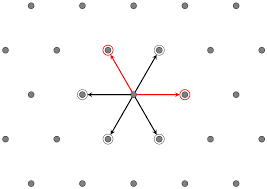
\includegraphics[width=0.5\textwidth]{A2.png}

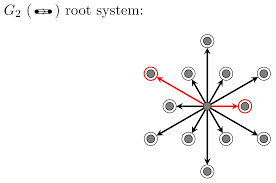
\includegraphics[width=0.5\textwidth]{G2.png}


% 6. Prove that Bℓ
% , ℓ ≥ 2 is isomorphic to the root system of so2ℓ+1.
% 1
\section{Root Systems of $\so_{2\ell+1}$}
\begin{prob}
    Prove that $B_\ell$, $\ell \geq 2$ is isomorphic to the root system of $\so_{2\ell+1}$.
\end{prob}

Let us recall that $\mathfrak{so}_{2n+1}$ can be represented by skew-symmetric $(2n+1)\times (2n+1)$ matrices. Specifically, we can choose a basis for $\mathfrak{so}_{2n+1}$ consisting of the elements
\[
M_{ij} \equiv E_{ij} - E_{ji}, \quad 1\leq i < j \leq 2n+1
\]
where $E_{ij}$ denotes the matrix with a $1$ in the $(i,j)$ entry and $0$ elsewhere. 


\begin{claim*}[Diagonalizing $\ad_{M_{ij}}$]
    The $\binom{2n+1}{2}$ eigenvectors of $\ad_{M_{ij}}$ are given by the following matrices (taking $i=1,j=2$ and $n=2$ for demonstration purposes):
    \[
        \begin{pmatrix}
            0&&1&&\\
            &0&\pm i&&\\
            -1&\mp i&0&&\\
            &&&0&\\
            &&&& 0
        \end{pmatrix},
        \begin{pmatrix}
            0&&&1&\\
            &0&&\pm i&\\
            &&0&& \\
            -1&\mp i&&0&\\
            &&&& 0
        \end{pmatrix},
        \begin{pmatrix}
            0&&&&1\\
            &0&&&\pm i\\
            &&0&& \\
            &&&0&\\
            -1&\mp i&&&0
        \end{pmatrix}
    \]
    (there are $2(2n-1)$ of these), in addition to the $\binom{2n-1}{2}+1$-dimensional
    kernel
    \[
    \begin{pmatrix}
        &c& \\
        -c & & \\
        & & \mathfrak{so}(2n-1)
    \end{pmatrix}
    \]
    Note that we have listed $2(2n-1)+\binom{2n-1}{2}+1 = \binom{2n+1}{2}$ eigenvectors, so these indeed form an eigenbasis.
\end{claim*}
\textit{Proof: } This can be verified by inspection or by multiplying out the matrices. It can be observed that everything in the first list has eigenvalue $\pm i$, while everything in the second list has eigenvalue $0$. $\Box$


\begin{claim*}[Definition of the Cartan subalgebra]
The set of matrices 
\[ H=\{ M_{12}, M_{34}, \cdots , M_{2n-1,2n} \} \]
forms a basis for the Cartan subalgebra of $\mathfrak{so}_{2n+1}$.
\end{claim*}
\textit{Proof: } It can be observed that the commutator of any matrix $M_{ij}$ with another matrix $M_{kl}$, where $i,j,k,l$ are distinct, results in a matrix of the form 
\[ 
\begin{pmatrix}
&c& \\
-c & & \\
& & \mathfrak{so}(2n-1)
\end{pmatrix}    
\]
This can be verified by explicitly calculating the commutation of $M_{ij}$ with $M_{kl}$
Therefore, it follows that the matrices $M_{12}, M_{34}, \cdots , M_{2n-1,2n}$
commute with each other. Furthermore, their joint kernel is is precisely
the span of $M_{12},\dots M_{2n-1,2n}$ indicating
that no additional elements can be added to the subalgebra. We already showed
that all of these
matrices are diagonalizable, so they form a basis for the Cartan subalgebra. $\Box$

Now we need to determine the roots of this Cartan subalgebra, which means we have to find their common eigenvectors and determine their corresponding eigenvalues. According to the second claim, consider matrices of the following form (for illustrative purposes, let's assume $n=2$):
\[ 
\begin{pmatrix}
0&&1&\pm_2 i&\\
&0&\pm_1 i&\pm_1 \mp_21&\\
-1&\mp_1 i&0&&\\
\mp_2 i&\pm_1\pm_21&&0&\\
&&&& 0
\end{pmatrix}    
\]
where we have four choices of $(\pm_1,\pm_2) \in \{1,-1\}^2$. The above matrix is an eigenvector of $\ad_{M_{12}}$ with eigenvalue $\pm_1 i$, and an eigenvector of $\ad_{M_{34}}$ with eigenvalue $\pm_2 i$. In general, when we consider different choices of $(\pm_1,\pm_2)$, the above matrix will have eigenvalues of $\pm_1 i$ and $\pm_2 i$ for two of the Cartan subalgebra basis elements, and will be in the kernel of all the other Cartan subalgebra basis elements. Therefore, we obtain roots of the form (expressing covectors in terms of the co-basis corresponding to our Cartan basis)
\[ \underbrace{(0,\cdots , 0 , \pm_1 i , 0 , \cdots , \pm_2 i , 0 , \cdots , 0)}_{\pm i\text{'s in any two positions}} \tag{$\star$}\]
There are $4\binom{n}{2}$ of these. Additionally, we have the eigenvectors of the form
(again, taking $n=2$ for demonstration purposes)
\[ 
\begin{pmatrix}
0&&&&1\\
&0&&&\pm i\\
&&0&&\\
&&&0&\\
-1&\mp i&&&0
\end{pmatrix}
\]
These eigenvectors have eigenvalue $\pm i$ with respect to $\ad_{M_{ij}}$ in the above example, and they are in the kernel of the remaining Cartan subalgebra elements. Therefore, we obtain roots of the form
\[ \underbrace{(0,\cdots , 0 , \pm i , 0 , \cdots , 0)}_{\pm i\text{ in any one position}} \tag{$\star\star$}\]
There are $2n$ of these. In addition to the $4\binom{n}{2}$ roots mentioned earlier, these roots complete the set of roots for the Cartan subalgebra. This can be verified by checking the dimensions: $2n+4\binom{n}{2}+n = \binom{2n+1}{2}$, which is the dimension of $\mathfrak{so}_{2n+1}$ (including the dimension of the Cartan subalgebra itself).\\

To complete the problem, we transfer the Killing form
from $\mathfrak{so}_{2n+1}$ to the Cartan subalgebra.
It is well-known that the Killing form of $\mathfrak{so}_{2n + 1}$
in our basis is $\kappa(X,Y) = (2n-1)\tr(XY)$ (e.g. repeat the proof
of problem $4$ on pset $4$),
i.e. $\kappa(M_{ij}, M_{kl}) = (2n-1)\left(\delta_{jk}\delta_{il} - \delta_{ik}\delta_{jl}\right)$.
The restriction to our Cartan subalgebra is
just $-(2n-1)$ identically. The constant factor
doesn't matter; what matters is that this is the standard
fully \textbf{negative} definite inner product on $\CC^n$.

Transferring this to the dual space, we see that this
corresponds to the fully \textbf{positive} definite inner product
as long as we rotate each root by $i$. Under this basis,
our roots can be written:
\begin{itemize}
    \item $\pm e_i \pm e_j$ for $i\neq j$ (roots of type $(\star)$).
    \item $\pm e_i$ for $i\neq j$ (roots of type $(\star\star)$).
\end{itemize}

This is precisely the root system of type $B_n$.
\end{document}